\subsection{PIMS Login Module}
This module is responsible for allowing a user to login into and logout out of Pentec Patient Information Management System. A user should login with the credentials they were assigned upon registration. If the user is not assigned a user name then an exception is thrown and the user is redirected to the login page. \par 

To avoid "Spambots", a reCAPTCHA challenge is used. 

\subsubsection{Scope}
The scope is shown in the use case diagram below: \par
\begin{figure}[H]
	\centerline{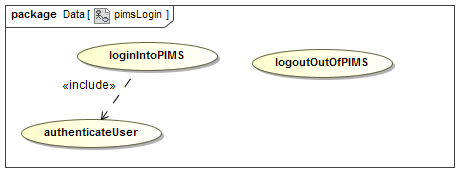
\includegraphics[width=0.75\linewidth]{./Functional_Requirements/Graphics/pimsLogin/pimsLogin}}
	\caption{Login module scope}
\end{figure}

\subsubsection{Use cases}
\begin{description}
	\item{\textbf{loginToPIMS -- [priority: critical] }}
	This use case is to cater for the logging in of user into the system. It entails the authentication of each user as well as their authorization, which is based on their access rights.
	\begin{description}
	\item{\textbf{Service Contract}} The service contract for loginToPIMS is shown below.
		\begin{figure}[H]
			\centerline{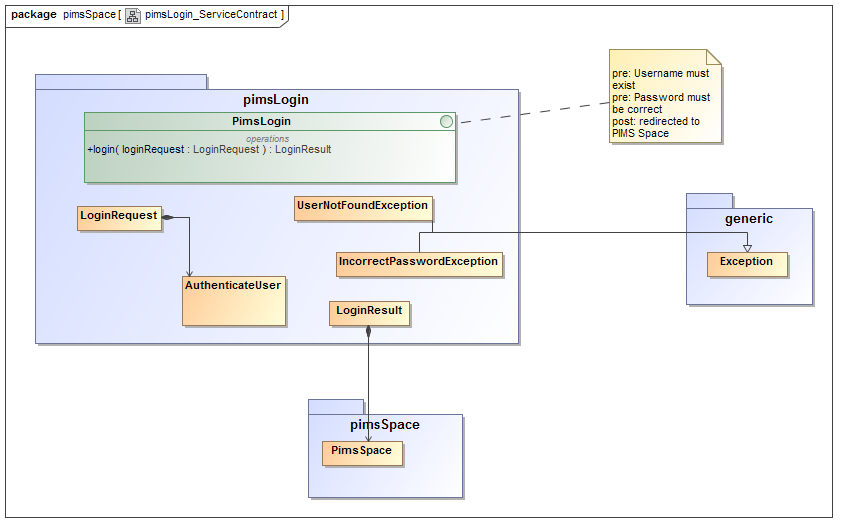
\includegraphics[width=0.7\linewidth]{./Functional_Requirements/Graphics/pimsLogin/pimsLogin_ServiceContract}}
			\caption{Service contract for pimsLogin}
		\end{figure}
	\end{description}
	\item{\textbf{logoutOfPIMS -- [priority: critical]}}
	This use case logs a user out of the system by destroying the session. The user will not be allowed access unless they log back in.
	\begin{description}
	\item{\textbf{Service Contract}} The service contract for logoutOfPIMS is shown below.
		\begin{figure}[H]
			\centerline{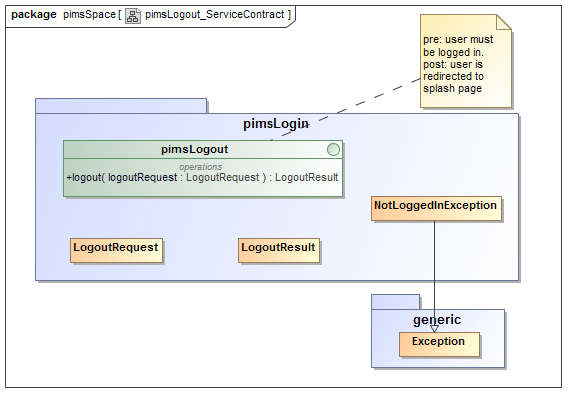
\includegraphics[width=0.7\linewidth]{./Functional_Requirements/Graphics/pimsLogin/pimsLogout_ServiceContract}}
			\caption{Service contract for logoutOfPIMS }
		\end{figure}
	\end{description}
	
		\item{\textbf{authenticateUser -- [priority: critical]}}
	This use case makes sure that only registered users can use PIMS. It also manages the user rights so that users only access what's intended for them. If a normal user tries to access admin pages, then they are redirected to a page that applies to their access rights.
\end{description}